\documentclass{standalone}
\usepackage{tikz}
\usetikzlibrary{patterns, positioning}

\begin{document}
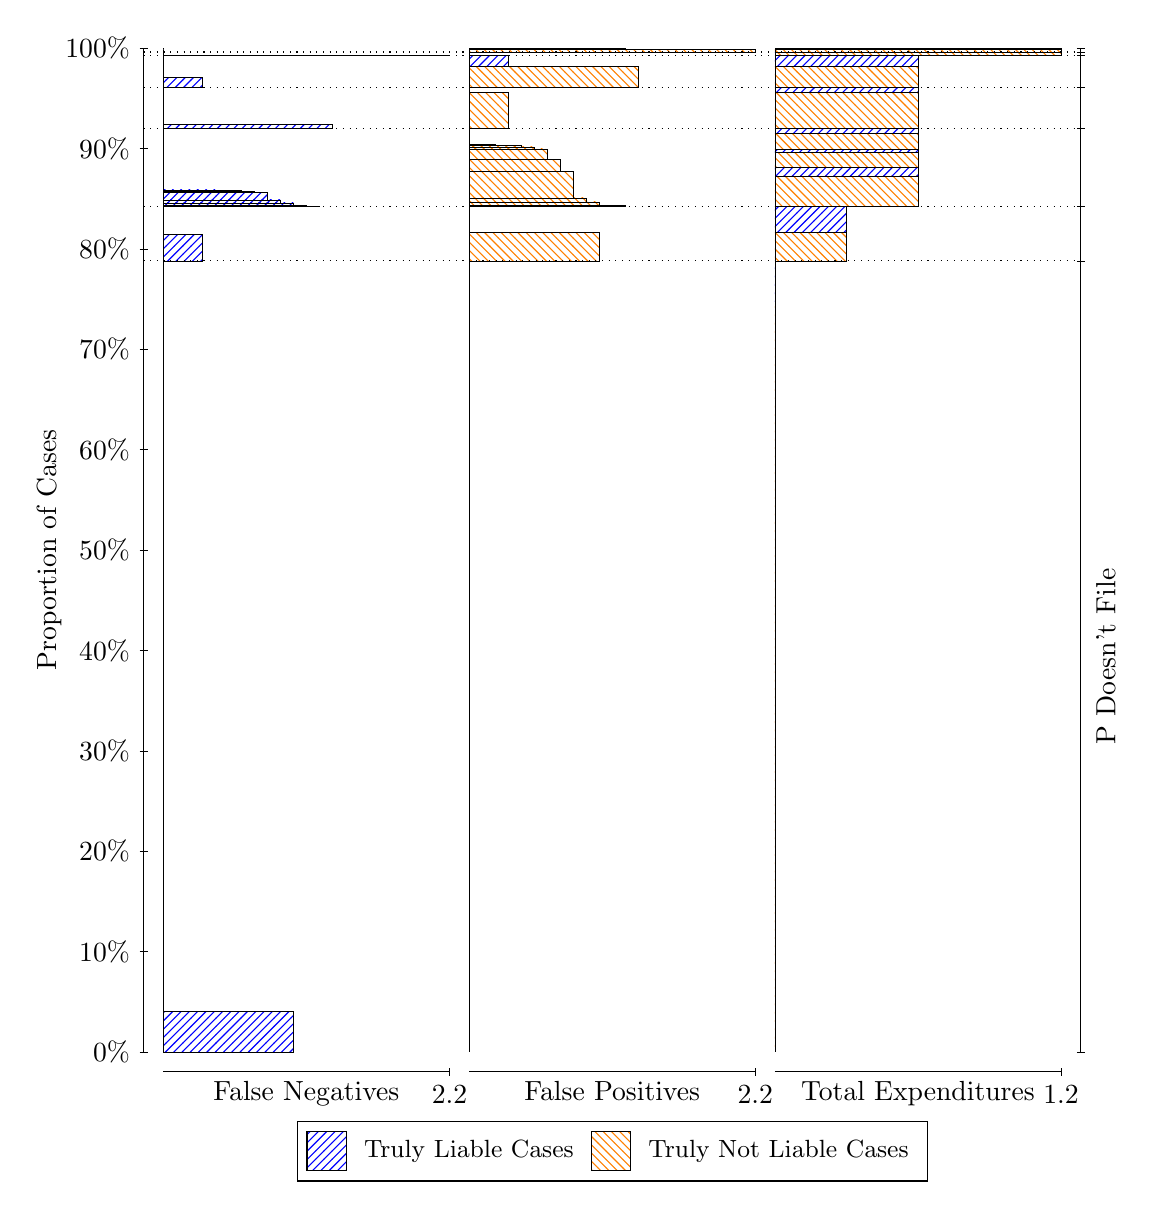
\begin{tikzpicture}
\draw[black, very thin] (1.5,1.75) -- (1.5,14.5);
\node[rotate=90, anchor=center] at (0.3, 8.125) {Proportion of Cases};
\draw[black, very thin] (1.45,1.75) -- (1.55,1.75);
\node[anchor=east] at (1.45, 1.75) {0\%};
\draw[black, very thin] (1.45,3.025) -- (1.55,3.025);
\node[anchor=east] at (1.45, 3.025) {10\%};
\draw[black, very thin] (1.45,4.3) -- (1.55,4.3);
\node[anchor=east] at (1.45, 4.3) {20\%};
\draw[black, very thin] (1.45,5.575) -- (1.55,5.575);
\node[anchor=east] at (1.45, 5.575) {30\%};
\draw[black, very thin] (1.45,6.85) -- (1.55,6.85);
\node[anchor=east] at (1.45, 6.85) {40\%};
\draw[black, very thin] (1.45,8.125) -- (1.55,8.125);
\node[anchor=east] at (1.45, 8.125) {50\%};
\draw[black, very thin] (1.45,9.4) -- (1.55,9.4);
\node[anchor=east] at (1.45, 9.4) {60\%};
\draw[black, very thin] (1.45,10.675) -- (1.55,10.675);
\node[anchor=east] at (1.45, 10.675) {70\%};
\draw[black, very thin] (1.45,11.95) -- (1.55,11.95);
\node[anchor=east] at (1.45, 11.95) {80\%};
\draw[black, very thin] (1.45,13.225) -- (1.55,13.225);
\node[anchor=east] at (1.45, 13.225) {90\%};
\draw[black, very thin] (1.45,14.5) -- (1.55,14.5);
\node[anchor=east] at (1.45, 14.5) {100\%};

\draw[black, very thin] (13.4,1.75) -- (13.4,14.5);
\draw[black, very thin] (13.35,1.75) -- (13.45,1.75);
\node[anchor=west] at (13.35, 1.75) {};
\draw[black, very thin] (13.35,11.797) -- (13.45,11.797);
\node[anchor=west] at (13.35, 11.797) {};
\draw[black, very thin] (13.35,12.491) -- (13.45,12.491);
\node[anchor=west] at (13.35, 12.491) {};
\draw[black, very thin] (13.35,13.475) -- (13.45,13.475);
\node[anchor=west] at (13.35, 13.475) {};
\draw[black, very thin] (13.35,13.996) -- (13.45,13.996);
\node[anchor=west] at (13.35, 13.996) {};
\draw[black, very thin] (13.35,14.402) -- (13.45,14.402);
\node[anchor=west] at (13.35, 14.402) {};
\draw[black, very thin] (13.35,14.449) -- (13.45,14.449);
\node[anchor=west] at (13.35, 14.449) {};
\draw[black, very thin] (13.35,14.5) -- (13.45,14.5);
\node[anchor=west] at (13.35, 14.5) {};

\draw[black, very thin, pattern color=blue, pattern=north east lines] (1.75,1.75) rectangle (3.4015,2.2704);
\draw[black, very thin, pattern color=orange, pattern=north west lines] (1.75,2.2704) rectangle (1.75,11.797);
\draw[black, very thin, pattern color=blue, pattern=north east lines] (1.75,11.797) rectangle (2.2455,12.13);
\draw[black, very thin, pattern color=orange, pattern=north west lines] (1.75,12.13) rectangle (1.75,12.491);
\draw[black, very thin, pattern color=blue, pattern=north east lines] (1.75,12.491) rectangle (3.7318,12.493);
\draw[black, very thin, pattern color=blue, pattern=north east lines] (1.75,12.493) rectangle (3.5667,12.5);
\draw[black, very thin, pattern color=blue, pattern=north east lines] (1.75,12.5) rectangle (3.4015,12.532);
\draw[black, very thin, pattern color=blue, pattern=north east lines] (1.75,12.532) rectangle (3.2364,12.533);
\draw[black, very thin, pattern color=blue, pattern=north east lines] (1.75,12.533) rectangle (3.2364,12.571);
\draw[black, very thin, pattern color=blue, pattern=north east lines] (1.75,12.571) rectangle (3.0712,12.663);
\draw[black, very thin, pattern color=blue, pattern=north east lines] (1.75,12.663) rectangle (2.9061,12.677);
\draw[black, very thin, pattern color=blue, pattern=north east lines] (1.75,12.677) rectangle (2.7409,12.69);
\draw[black, very thin, pattern color=blue, pattern=north east lines] (1.75,12.69) rectangle (2.5758,12.694);
\draw[black, very thin, pattern color=blue, pattern=north east lines] (1.75,12.694) rectangle (2.4106,12.698);
\draw[black, very thin, pattern color=orange, pattern=north west lines] (1.75,12.698) rectangle (1.75,13.475);
\draw[black, very thin, pattern color=blue, pattern=north east lines] (1.75,13.475) rectangle (3.897,13.534);
\draw[black, very thin, pattern color=orange, pattern=north west lines] (1.75,13.534) rectangle (1.75,13.996);
\draw[black, very thin, pattern color=blue, pattern=north east lines] (1.75,13.996) rectangle (2.2455,14.129);
\draw[black, very thin, pattern color=orange, pattern=north west lines] (1.75,14.129) rectangle (1.75,14.402);
\draw[black, very thin, pattern color=blue, pattern=north east lines] (1.75,14.402) rectangle (5.3833,14.405);
\draw[black, very thin, pattern color=orange, pattern=north west lines] (1.75,14.405) rectangle (1.75,14.449);
\draw[black, very thin, pattern color=orange, pattern=north west lines] (1.75,14.449) rectangle (1.75,14.481);
\draw[black, very thin, pattern color=blue, pattern=north east lines] (1.75,14.481) rectangle (1.75,14.5);
\draw[black, very thin, pattern color=orange, pattern=north west lines] (5.6333,1.75) rectangle (5.6333,11.277);
\draw[black, very thin, pattern color=blue, pattern=north east lines] (5.6333,11.277) rectangle (5.6333,11.797);
\draw[black, very thin, pattern color=orange, pattern=north west lines] (5.6333,11.797) rectangle (7.2848,12.159);
\draw[black, very thin, pattern color=blue, pattern=north east lines] (5.6333,12.159) rectangle (5.6333,12.491);
\draw[black, very thin, pattern color=orange, pattern=north west lines] (5.6333,12.491) rectangle (7.6152,12.499);
\draw[black, very thin, pattern color=orange, pattern=north west lines] (5.6333,12.499) rectangle (7.45,12.506);
\draw[black, very thin, pattern color=orange, pattern=north west lines] (5.6333,12.506) rectangle (7.2848,12.547);
\draw[black, very thin, pattern color=orange, pattern=north west lines] (5.6333,12.547) rectangle (7.1197,12.597);
\draw[black, very thin, pattern color=orange, pattern=north west lines] (5.6333,12.597) rectangle (6.9545,12.935);
\draw[black, very thin, pattern color=orange, pattern=north west lines] (5.6333,12.935) rectangle (6.7894,13.086);
\draw[black, very thin, pattern color=orange, pattern=north west lines] (5.6333,13.086) rectangle (6.6242,13.22);
\draw[black, very thin, pattern color=orange, pattern=north west lines] (5.6333,13.22) rectangle (6.4591,13.245);
\draw[black, very thin, pattern color=orange, pattern=north west lines] (5.6333,13.245) rectangle (6.2939,13.268);
\draw[black, very thin, pattern color=blue, pattern=north east lines] (5.6333,13.268) rectangle (5.9636,13.272);
\draw[black, very thin, pattern color=blue, pattern=north east lines] (5.6333,13.272) rectangle (5.7985,13.276);
\draw[black, very thin, pattern color=blue, pattern=north east lines] (5.6333,13.276) rectangle (5.6333,13.475);
\draw[black, very thin, pattern color=orange, pattern=north west lines] (5.6333,13.475) rectangle (6.1288,13.937);
\draw[black, very thin, pattern color=blue, pattern=north east lines] (5.6333,13.937) rectangle (5.6333,13.996);
\draw[black, very thin, pattern color=orange, pattern=north west lines] (5.6333,13.996) rectangle (7.7803,14.268);
\draw[black, very thin, pattern color=blue, pattern=north east lines] (5.6333,14.268) rectangle (6.1288,14.402);
\draw[black, very thin, pattern color=orange, pattern=north west lines] (5.6333,14.402) rectangle (5.6333,14.446);
\draw[black, very thin, pattern color=blue, pattern=north east lines] (5.6333,14.446) rectangle (5.6333,14.449);
\draw[black, very thin, pattern color=orange, pattern=north west lines] (5.6333,14.449) rectangle (9.2667,14.481);
\draw[black, very thin, pattern color=blue, pattern=north east lines] (5.6333,14.481) rectangle (7.6152,14.5);
\draw[black, very thin, pattern color=orange, pattern=north west lines] (9.5167,1.75) rectangle (9.5167,11.277);
\draw[black, very thin, pattern color=blue, pattern=north east lines] (9.5167,11.277) rectangle (9.5167,11.797);
\draw[black, very thin, pattern color=orange, pattern=north west lines] (9.5167,11.797) rectangle (10.425,12.159);
\draw[black, very thin, pattern color=blue, pattern=north east lines] (9.5167,12.159) rectangle (10.425,12.491);
\draw[black, very thin, pattern color=orange, pattern=north west lines] (9.5167,12.491) rectangle (11.333,12.877);
\draw[black, very thin, pattern color=blue, pattern=north east lines] (9.5167,12.877) rectangle (11.333,12.985);
\draw[black, very thin, pattern color=orange, pattern=north west lines] (9.5167,12.985) rectangle (11.333,13.171);
\draw[black, very thin, pattern color=blue, pattern=north east lines] (9.5167,13.171) rectangle (11.333,13.213);
\draw[black, very thin, pattern color=orange, pattern=north west lines] (9.5167,13.213) rectangle (11.333,13.418);
\draw[black, very thin, pattern color=blue, pattern=north east lines] (9.5167,13.418) rectangle (11.333,13.475);
\draw[black, very thin, pattern color=orange, pattern=north west lines] (9.5167,13.475) rectangle (11.333,13.937);
\draw[black, very thin, pattern color=blue, pattern=north east lines] (9.5167,13.937) rectangle (11.333,13.996);
\draw[black, very thin, pattern color=orange, pattern=north west lines] (9.5167,13.996) rectangle (11.333,14.268);
\draw[black, very thin, pattern color=blue, pattern=north east lines] (9.5167,14.268) rectangle (11.333,14.402);
\draw[black, very thin, pattern color=orange, pattern=north west lines] (9.5167,14.402) rectangle (13.15,14.446);
\draw[black, very thin, pattern color=blue, pattern=north east lines] (9.5167,14.446) rectangle (13.15,14.449);
\draw[black, very thin, pattern color=orange, pattern=north west lines] (9.5167,14.449) rectangle (13.15,14.481);
\draw[black, very thin, pattern color=blue, pattern=north east lines] (9.5167,14.481) rectangle (13.15,14.5);
\draw[black, dotted] (1.5,11.797) -- (13.4,11.797);
\draw[black, dotted] (1.5,12.491) -- (13.4,12.491);
\draw[black, dotted] (1.5,13.475) -- (13.4,13.475);
\draw[black, dotted] (1.5,13.996) -- (13.4,13.996);
\draw[black, dotted] (1.5,14.402) -- (13.4,14.402);
\draw[black, dotted] (1.5,14.449) -- (13.4,14.449);
\draw[black, very thin] (1.75,1.5) -- (5.3833,1.5);
\node[anchor=north] at (3.5667, 1.5) {False Negatives};
\draw[black, very thin] (5.3833,1.45) -- (5.3833,1.55);
\node[anchor=north] at (5.3833, 1.45) {2.2};

\draw[black, very thin] (5.6333,1.5) -- (9.2667,1.5);
\node[anchor=north] at (7.45, 1.5) {False Positives};
\draw[black, very thin] (9.2667,1.45) -- (9.2667,1.55);
\node[anchor=north] at (9.2667, 1.45) {2.2};

\draw[black, very thin] (9.5167,1.5) -- (13.15,1.5);
\node[anchor=north] at (11.333, 1.5) {Total Expenditures};
\draw[black, very thin] (13.15,1.45) -- (13.15,1.55);
\node[anchor=north] at (13.15, 1.45) {1.2};

\node[black, centered, rotate=90] at (13.72, 6.7737) {P Doesn't File};







\draw (7.449999999999999,1.5) node[draw=none] (baseCoordinate) {};
\begin{scope}[align=center]
        \matrix[scale=0.5, draw=black, below=0.5cm of baseCoordinate, nodes={draw}, column sep=0.1cm]{
            \node[rectangle, draw, minimum width=0.5cm, minimum height=0.5cm, pattern=north east lines, pattern color=blue] {}; &
            \node[draw=none, font=\small] (B) {Truly Liable Cases}; &
            \node[rectangle, draw, minimum width=0.5cm, minimum height=0.5cm, pattern=north west lines, pattern color=orange] {}; &
            \node[draw=none, font=\small] (B) {Truly Not Liable Cases}; \\
            };
\end{scope}

\end{tikzpicture}
\end{document}